\documentclass[a4paper,11pt]{article}
\usepackage[latin1]{inputenc}
\usepackage[T1]{fontenc}
\usepackage{bbm}
\usepackage{amsmath}
\usepackage{indentfirst}
\usepackage{fullpage}
\usepackage{url}
\usepackage{geometry}
\geometry{verbose,tmargin=3cm,bmargin=2cm,lmargin=2cm,rmargin=2cm}
\usepackage{graphicx}
\usepackage[center,footnotesize]{caption}
\usepackage[section]{placeins}
\usepackage{subfig}

\DeclareRobustCommand{\greektext}{%
  \fontencoding{LGR}\selectfont\def\encodingdefault{LGR}}
\DeclareRobustCommand{\textgreek}[1]{\leavevmode{\greektext #1}}
\DeclareFontEncoding{LGR}{}{}
\DeclareTextSymbol{\~}{LGR}{126}

\title{Series 4}
\date{October 11, 2011}
\author{Genomics and bioinformatics - Week 4}

\begin{document}
\maketitle

\section{Sequence alignment}
The Needlman-Wunsch algorithm uses a method called ``dynamic programming''. This is a very general programming technique. It involves three main steps,
\begin{enumerate}
\item Initialization
\item Scoring (matrix fill)
\item Alignment (backtracking)
\end{enumerate}

In the first exercise of this session you will manually perform a global alignment of two sequences based on the following scoring scheme,

\emph{Match:} \texttt{+1}, \emph{Mismatch:} \texttt{-1}, \emph{Gap:} \texttt{-2}\\

Sequence 1: \texttt{GAATTCAGA}

Sequence 2: \texttt{GGATCGA}.

\begin{center}
\includegraphics[width=0.8\textwidth]{matrix.png}
\end{center}

Solution:\\

\section{Pair HMM}

In this exercise, we will construct a pair Hiden Markov Model for
the same sequences as in the first exercise and align them using the
path with maximum probabiity.

The maximum probability of generating the alignment and the corresponding path are calculated by a dynamic
programming algorithm which is called the Viterbi Algorithm. You will
see during the exercise that the Viterbi algorithm is actually similar
to the Needleman-Wunsch algorthm.
\vspace{0.5cm}


The algorithm goes through the three steps

Step1: Intialization

Step2: Recursion

Step3: Termination

\vspace{0.5cm}

A general pair HMM is shown in Figure 1. Pair HMM consists of the following parameters,
\begin{figure}
\begin{centering}
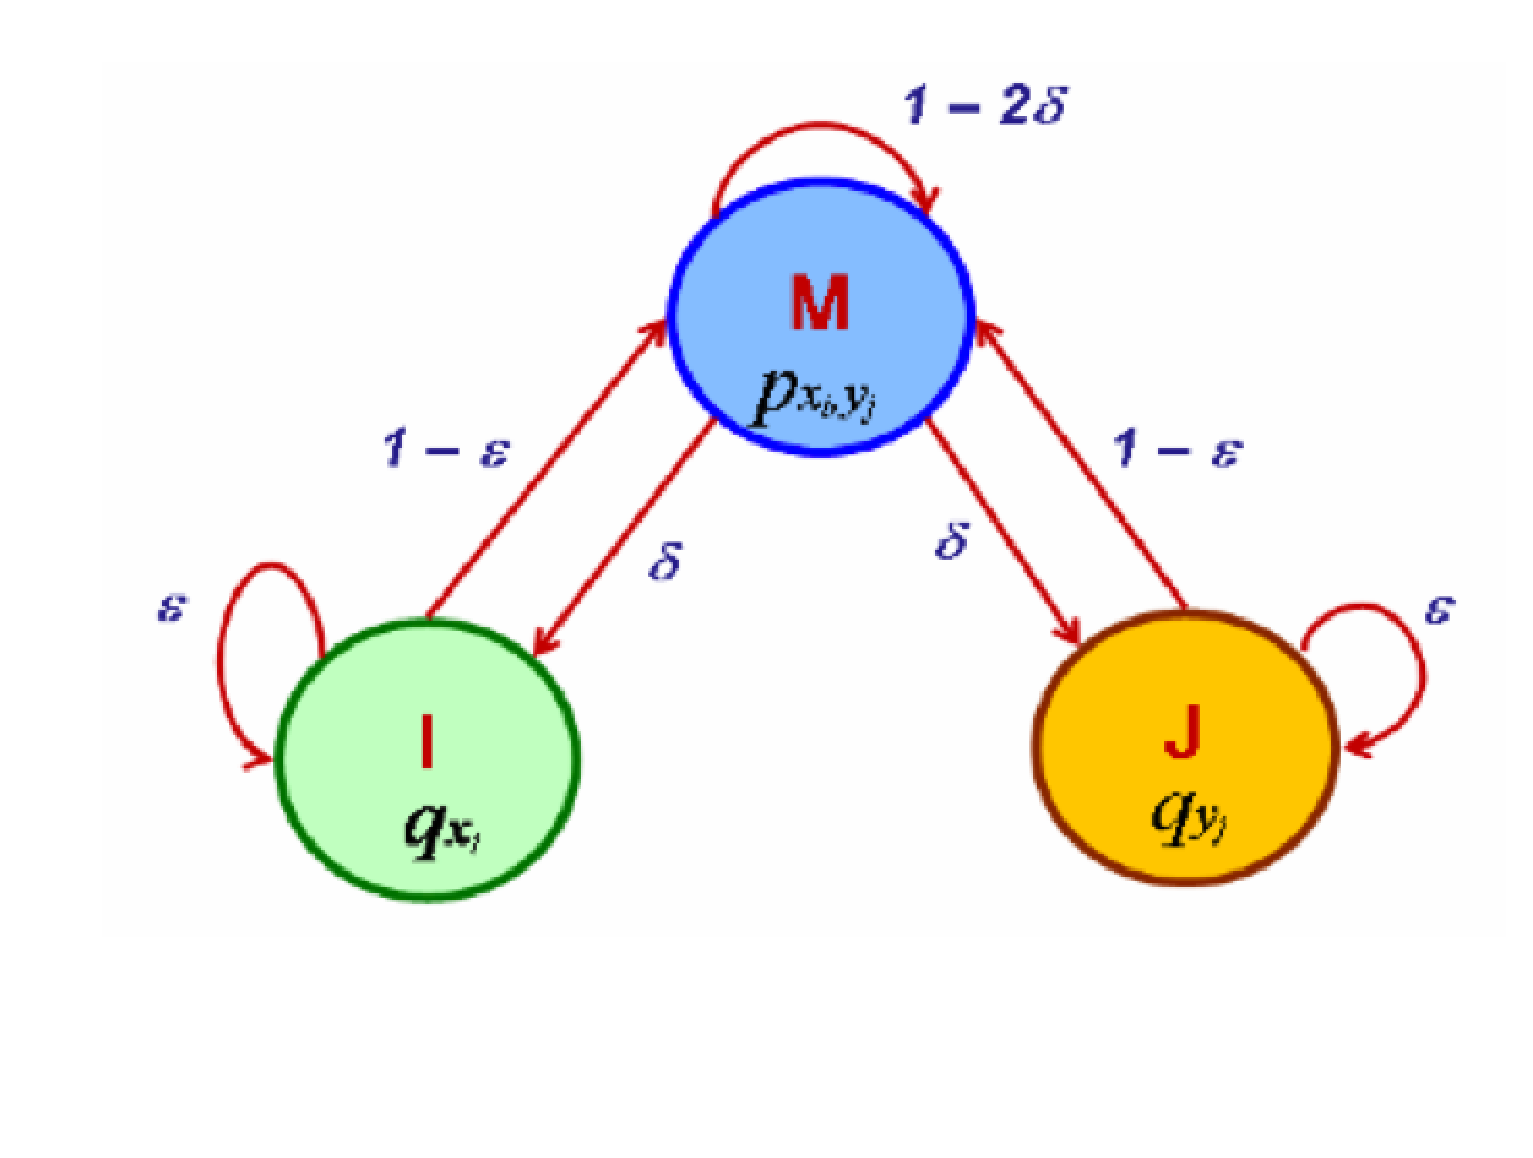
\includegraphics[width=4in]{HMMfigures}\caption{Pair Hidden Markov Model}
\par\end{centering}
\end{figure}

\vspace{0.5cm}

Three states: M, I, J .

State M matches one letter from each sequence

State I inserts a gap in the second sequence 

State J inserts a gap in the first sequence

\vspace{0.5cm}

Emission probabilities: p(x y), q(x) and q(y), where,

p (x,y) = probability of emitting a pair of characters {[}x,y{]} 

qx = probabilityof emitting a pair of character {[}x,\_{]}

qy = probability of emitting a pair of characters{[}\_,y{]}

\vspace{0.5cm}

Transition probabilities:

\textgreek{d} = probability of opening a gap 

\textgreek{e} = probability of extending a gap 

\end{document}